% 0440(본책 80쪽) — 지름 AB 인 반원 O, 현 AC·BD 의 연장선의 교점 P, OC·OD, ∠COD=30°, ∠APB=x. 답(x)은 적지 않는다. 스캔 삽화를 TikZ 로 다시 그림.
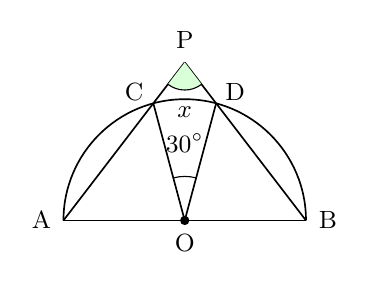
\begin{tikzpicture}[scale=1.4, line width=0.6pt]
  \draw (1.100,0.000) arc (0:180:1.100);
  \draw (-1.100,0.000) -- (1.100,0.000);
  \draw (-1.100,0.000) -- (0.000,1.434);
  \draw (1.100,0.000) -- (0.000,1.434);
  \draw (0.000,0.000) -- (-0.285,1.063);
  \draw (0.000,0.000) -- (0.285,1.063);
  \fill (0.000,0.000) circle (1.2pt);
  \fill[green!15] (0.000,1.434) -- (-0.152,1.235) arc (232.5:307.5:0.250) -- cycle;
  \draw[line width=0.4pt] (-0.152,1.235) arc (232.5:307.5:0.250);
  \draw[line width=0.4pt] (0.104,0.386) arc (75.0:105.0:0.400);
  \node[font=\small, inner sep=0.5pt] at (-0.000,0.984) {$x$};
  \node[font=\small, inner sep=0.5pt] at (0.000,0.700) {$30^\circ$};
  \node[font=\small, inner sep=1.5pt] at (-1.300,0.000) {A};
  \node[font=\small, inner sep=1.5pt] at (1.300,0.000) {B};
  \node[font=\small, inner sep=1.5pt] at (-0.458,1.163) {C};
  \node[font=\small, inner sep=1.5pt] at (0.458,1.163) {D};
  \node[font=\small, inner sep=1.5pt] at (0.000,1.634) {P};
  \node[font=\small, inner sep=1.5pt] at (-0.000,-0.200) {O};
\end{tikzpicture}
